% Define the page style
\fancypagestyle{chapterstyle}{
   \fancyhead[L]{\nouppercase{\rightmark}}
   \fancyhead[R]{Projet de fin d'etudes 2023-2024}
   \fancyfoot[C]{\vspace{20pt}\thepage} % Adjust the vertical space here
   \setlength{\headheight}{20pt}
   \setlength{\footskip}{30pt} % Adjust the value as needed
}





\chapter{Implémentation et Validation}
\pagestyle{chapterstyle}
Dans la suite du projet, l'implémentation et la validation 
sont d'une importance capitale. Le choix des outils de 
développement impacte significativement le temps nécessaire à 
la programmation et la qualité du produit final. Cette phase 
consiste à concrétiser le modèle conceptuel précédemment établi 
en composants logiciels formant notre système, puis à vérifier 
leur bon fonctionnement. Dans ce chapitre, nous allons présenter 
de manière succincte les différents outils que nous avons utilisés 
tout au long du développement et de la validation de notre 
application.
Ainsi le travail réalisé.

\newpage
\vspace{1cm}

\section{Outils et technologies de développement}
\subsection{Outils de conception}

\large 
\textbf{Figma}

\begin{figure}[htbp]
   \centering
   \includegraphics[scale=0.03]{Images/figma.png} 
   \caption{Logo Figma}
   \label{fig:figma}
\end{figure}
Figma est un outil de design collaboratif en ligne pour la création d'interfaces utilisateur. Il permet de créer des maquettes et des prototypes interactifs, facilitant la collaboration en temps réel. Avec des fonctionnalités avancées comme le partage de projets, les commentaires et l'édition simultanée, Figma améliore la communication et l'efficacité du design. Il est essentiel pour visualiser, tester et affiner les concepts avant le développement final.
\newline

\large 
\textbf{Lucidchart}
\begin{figure}[htbp]
   \centering
   \includegraphics[scale=0.2]{Images/lucid.jpeg} 
   \caption{Logo Lucidchart}
   \label{fig:lucid}
\end{figure}

Lucidchart est un outil en ligne pour créer et partager des diagrammes et des visualisations de données. Il permet de dessiner des diagrammes de flux, des organigrammes, des cartes conceptuelles, et bien d'autres schémas. Ses fonctionnalités collaboratives permettent à plusieurs utilisateurs de travailler simultanément, améliorant ainsi la communication et la coordination. Lucidchart est idéal pour représenter visuellement des processus complexes, organiser des informations et planifier des projets.

\subsection{Environnement de développement}
\large 
\textbf{Visual Studio Code}

\begin{figure}[htbp]
   \centering
   \includegraphics[scale=0.06]{Images/vs.png} 
   \caption{Logo Visual Stduio Code}
   \label{fig:vscode}
\end{figure}

Visual Studio Code est éditeur de texte open source, gratuit et multiplateforme (Windows, Mac et Linux), développé
par Microsoft. Principalement conçu pour le développement
d’application avec JavaScript, Type script et Node.js, l’éditeur peut s’adapter à d’autres types de langages grâce à un
Système d’extension bien fourni.
\newline

\large 
\textbf{4D Client}

\begin{figure}[htbp]
   \centering
   \includegraphics[scale=0.2]{Images/4dcl.png} 
   \caption{Logo 4D Client}
   \label{fig:4dcl}
\end{figure}

4D vous permet de construire des applications client-serveur 
personnalisées qui sont homogènes, multiplateformes et avec 
une option de mise à jour automatique. Les applications 
client et serveur sont configurées dans la page Client/Serveur 
de la boîte de dialogue Construire une application.
\newline

\large 
\textbf{4D Serveur}

\begin{figure}[htbp]
   \centering
   \includegraphics[scale=0.2]{Images/4dsrv.png} 
   \caption{Logo 4D Serveur}
   \label{fig:4dsrv}
\end{figure}

4D Server est un composant logiciel de la plateforme de développement 4D qui permet le déploiement et la gestion
d’applications client-sebrveur. Il offre un environnement robuste et évolutif pour héberger des applications 4D, 
permettant à plusieurs utilisateurs d’y accéder et d’interagir avec
l’application simultanément. 4D Server agit comme un hub centralisé, 
gérant le stockage des données, le traitement et la communication entre 
le serveur et les applications clientes connectées. Il prend en charge 
des fonctionnalités telles que l’accès simultané aux données partagées, 
la gestion des transactions, les contrôles de sécurité et la collaboration
multi-utilisateur.
\newline


\large 
\textbf{Postman}

\begin{figure}[htbp]
   \centering
   \includegraphics[scale=0.4]{Images/postman.png} 
   \caption{Logo postman}
   \label{fig:4dsrv}
\end{figure}

Postman fournit une interface conviviale où les développeurs 
peuvent spécifier les paramètres de requête, les entêtes, 
les corps de requête, les méthodes HTTP, etc. Ils peuvent 
également inspecter les réponses des serveurs, valider les 
résultats et effectuer des tests automatisés pour s’assurer que 
l’API fonctionne correctement. 
\newline

\large 
\textbf{GitLab}

\begin{figure}[htbp]
   \centering
   \includegraphics[scale=0.6]{Images/gitlab.jpg} 
   \caption{Logo GitLab}
   \label{fig:gitlab}
\end{figure}
GitLab est une plateforme DevOps complète proposée sous la forme 
d’une application unique. Elle révolutionne le développement, 
la sécurité, l’exploitation et la collaboration entre les équipes. 
Créez, testez et déployez des logiciels plus rapidement en 
n’utilisant qu’une seule solution. 

\subsection{Langages de développement}
\large 
\textbf{4D}

\begin{figure}[htbp]
   \centering
   \includegraphics[scale=0.8]{Images/logo-4d.jpg} 
   \caption{Logo 4D}
   \label{fig:4D}
\end{figure}
Le langage 4D est un langage de programmation spécifique à la
 plateforme utilisé dans l’environnement de développement 4D pour
  créer des applications professionnelles et des bases de données. 
  Il est conçu pour simplifier le développement d’applications 
  en fournissant des fonctionnalités spécifiques à la gestion des 
  données et des interfaces utilisateur.

\large 
\textbf{TypeScript}
\begin{figure}[h]
   \centering
   \includegraphics[scale=0.05]{Images/ts.png} 
   \caption{Logo TypeScript}
   \label{fig:ts}
\end{figure}

TypeScript, développé par Microsoft, est un surensemble de 
JavaScript qui ajoute des types statiques, permettant de détecter 
les erreurs dès la phase de développement. Il compile en JavaScript 
standard et est compatible avec tous les navigateurs. 
TypeScript offre des fonctionnalités avancées comme les 
interfaces, les énumérations et les génériques, et bénéficie 
d'un excellent support des outils de développement, facilitant 
l'auto-complétion et la refactorisation. Il est idéal pour les 
applications à grande échelle où la qualité du code est importante.
\newline

\large
\textbf{HTML}
\begin{figure}[htbp]
   \centering
   \includegraphics[scale=0.2]{Images/html.png} 
   \caption{Logo HTML}
   \label{fig:html}
\end{figure}

HTML est un langage de balisage conçu pour représenter les pages
 web. C’est un langage permettant d’écrire de l’hypertexte, 
 d’où son nom. HTML permet également de structurer sémantiquement 
 et logiquement et de mettre en forme le contenu des pages, 
 d’inclure des ressources multimédias dont des images, des 
 formulaires de saisie et des programmes informatiques.

 

\subsection{Frameworks}
\large
\textbf{React}
\begin{figure}[htbp]
   \centering
   \includegraphics[scale=0.1]{Images/react.png} 
   \caption{Logo React}
   \label{fig:react}
\end{figure}

React est une bibliothèque JavaScript frontale open source 
permettant de créer des interfaces utilisateur ou des composants 
d’interface utilisateur. Il est maintenu par Fa- cebook et une 
communauté de développeurs individuels et d’entreprises. React 
peut être utilisé comme base dans le dé- veloppement d’applications 
monopages ou mobiles.
\newline

\large
\textbf{Tailwind}
\begin{figure}[htbp]
   \centering
   \includegraphics[scale=0.6]{Images/tailwind.png} 
   \caption{Logo Tailwind}
   \label{fig:tailwind}
\end{figure}

Tailwind est un framework CSS qui fournit un catalogue complet de 
classes et d’outils CSS qui vous permet de commencer facilement 
à styliser votre site Web ou votre application.
\newline

\large
\textbf{Cypress}
\begin{figure}[htbp]
   \centering
   \includegraphics[scale=0.6]{Images/cy.jpg} 
   \caption{Logo Cypress}
   \label{fig:4D}
\end{figure}

Cypress est un framework de test open-source populaire utilisé 
pour automatiser les tests d’applications web. Il permet aux 
développeurs d’écrire des tests end-to-end (de bout en bout) pour 
vérifier le bon fonctionnement des applications web.

% travail realise
\section{Travail résalisé}
Cette section présente des captures d'écran de diverses interfaces de notre application, accompagnées de descriptions  détaillées.  Chaque  capture  illustre une interface spécifique de l'application et met en avant les fonctionnalités principales disponibles. Les descriptions fournissent des informations sur la disposition de l'interface, les boutons et les menus pertinents, ainsi que sur les actions que les utilisateurs peuvent réaliser.
\subsection{Page d'accueil}

La page  d’accueil est  conçue pour offrir une expérience utilisateur intuitive et informative. En haut une  barre  de navigation claire avec le logo de l’application et des liens vers les principales sections comme le bouton “sign in” qui permet l’utilisateur de  naviguer vers la page d’authentification. La section principale attire immédiatement l’attention avec un message accrocheur et une illustration attrayante, présentant l'objectif de la  plateforme. Les catégories d’emploi sont mises en  avant. Une section de guide des utilisateurs à travers des étapes simples de candidature. Un appel à l’action “Ready to start ?”  encourage l'engagement, en  redirigeant l’utilisateur vers le formulaire de  l’inscription. 
\begin{figure}[htbp]
   \centering
   \includegraphics[scale=0.6]{screens/accueil2.jpg} 
   \caption{Page d'accueil}
   \label{fig:accueil}
\end{figure}

\vspace{2cm}
\subsection{Authentification}
En cliquant le bouton “Sign In”, l’utilisateur sera redirigé vers la page d’authentification, contenant un formulaire basé sur React et Tailwind. Les utilisateurs peuvent saisir leurs  informations  d’identification, leur Email utilisateur et leur mot de passe, dans les champs correspondants. Le formulaire utilise la  méthode  POST  pour  envoyer  les données au  serveur. Du  côté serveur, une  application backend en  4D  est  chargée de recevoir les données, les vérifier  et les valider. Si les données sont valides, l’utilisateur va accéder vers son espace personnel, en dépendant de son rôle.
\newline
\begin{figure}[htbp]
   \centering
   \includegraphics[scale=0.5]{screens/signin.jpg} 
   \caption{Page d'authentification}
   \label{fig:accueil}
\end{figure}

Si les informations sont incorrectes, un message d’erreur "Wrong Email or Password" sera affiché. Si l’utilisateur oublie son mot de passe, il peut le réinitialiser en cliquant sur la fonctionnalité "Forgot Password  ?",  qui  le redirigera vers une autre page illustrée par la figure suivante. Sur cette page, il pourra remplir son  email. Une  fois soumis par  la  méthode POST, l'application backend de 4D vérifiera immédiatement la présence de l'adresse email dans sa base de données. Si elle n'est pas trouvée, un message d’erreur sera affiché.
\newline
\begin{figure}[htbp]
   \centering
   \includegraphics[scale=0.6]{screens/forgot.jpg} 
   \caption{Oublier le mot de passe}
   \label{fig:forgotPass}
\end{figure}

Sinon, si  l'email est  trouvé, un  courriel sera envoyé à l'adresse fournie via la méthode POST, contenant le  nouveau mot de  passe, comme illustré dans la figure.
\begin{figure}[htbp]
   \centering
   \includegraphics[scale=0.5]{screens/mailPssword.jpg} 
   \caption{Exemple d'un Email pour réintialiser le mot de passe}
   \label{fig:mailPass}
\end{figure}

\subsection{Espace Candidat}
\subsubsection{La page d’ inscription}
Le candidat peut accéder au formulaire d’inscription à partir du bouton “Ready to start” ou le bouton “Sign up” de la page d’authentification. Ce forumulaire comme il est représenté sur la figure 59. À droite, la section pour l'inscription comporte des champs de formulaire pour entrer des informations personnelles, y compris le prénom, le nom, le courriel, le mot de  passe, et  le numéro de téléphone. En bas, un bouton "REGISTER” permet de finaliser l'inscription. Juste en dessous, il y a un lien "Already have an account ? Sign In" pour rediriger les utilisateurs vers la page de connexion s’ils ont déjà un compte.

\begin{figure}[htbp]
   \centering
   \includegraphics[scale=0.5]{screens/signup.jpg} 
   \caption{Page d'inscription}
   \label{fig:singup}
\end{figure}

\subsubsection{Profil}
Après authentification, chaque utilisateur se voit attribuer un  rôle (candidat, recruteur ou administrateur),  qui  détermine  l'accès  à son  espace dédié. Prenons d'abord le cas où l'utilisateur est un candidat : il est redirigé directement vers son profil, comme illustré à la figure.
\newline

Dans la première section de son profil, le  candidat peut mettre à jour sa photo et ses informations personnelles. Dans la  deuxième section, il  peut ajouter ou mettre à jour son CV et sa lettre  de  motivation.  Enfin,  dans  la  dernière section, il a la possibilité de réinitialiser son mot de passe pour la plateforme. Toutes ces modifications se font grâce à la méthode POST/UPDATE.
\newline


\begin{figure}[htbp]
   \centering
   \includegraphics[scale=0.3]{screens/profile.png} 
   \caption{Profil}
   \label{fig:profile}
\end{figure}

\vspace{6cm}

\subsubsection{Postuler à une offre}
En naviguant via le menu de gauche, un simple clic sur le bouton "Offres" conduit à la page représentée par la figure .  Cette  page  présente plusieurs cartes, chacune décrivant une  offre d'emploi active, non  archivée, et  publiée par un recruteur. Chaque carte comprend les détails suivants : le titre du poste, la localisation, une brève description du poste, le  type de  contrat (stage, emploi, etc.), et le mode de travail (hybride, sur site, télétravail). En haut de la page, un menu permet de filtrer les offres d'emploi par domaine, tel que DevOps, Data science, et software engineering.
\newline

Chaque page affiche jusqu'à 6 cartes,  avec  une  fonction  de  pagination pour accéder aux offres suivantes.
\begin{figure}[htbp]
   \centering
   \includegraphics[scale=0.2]{screens/Offfers.png} 
   \caption{Liste des offres}
   \label{fig:listOffers}
\end{figure}

Comme illustré dans la figure, chaque carte est dotée de deux boutons. Le premier, intitulé "More", permet au candidat d'accéder à une page détaillant l'offre. Sur cette page, sont présentés  le  titre  de  l'offre,  sa  localisation,  son mode de travail, le type de contrat, la description du  poste,  ainsi  que  les exigences spécifiques du poste, comme illustré dans la figure
\newline
\begin{figure}[htb]
   \centering
   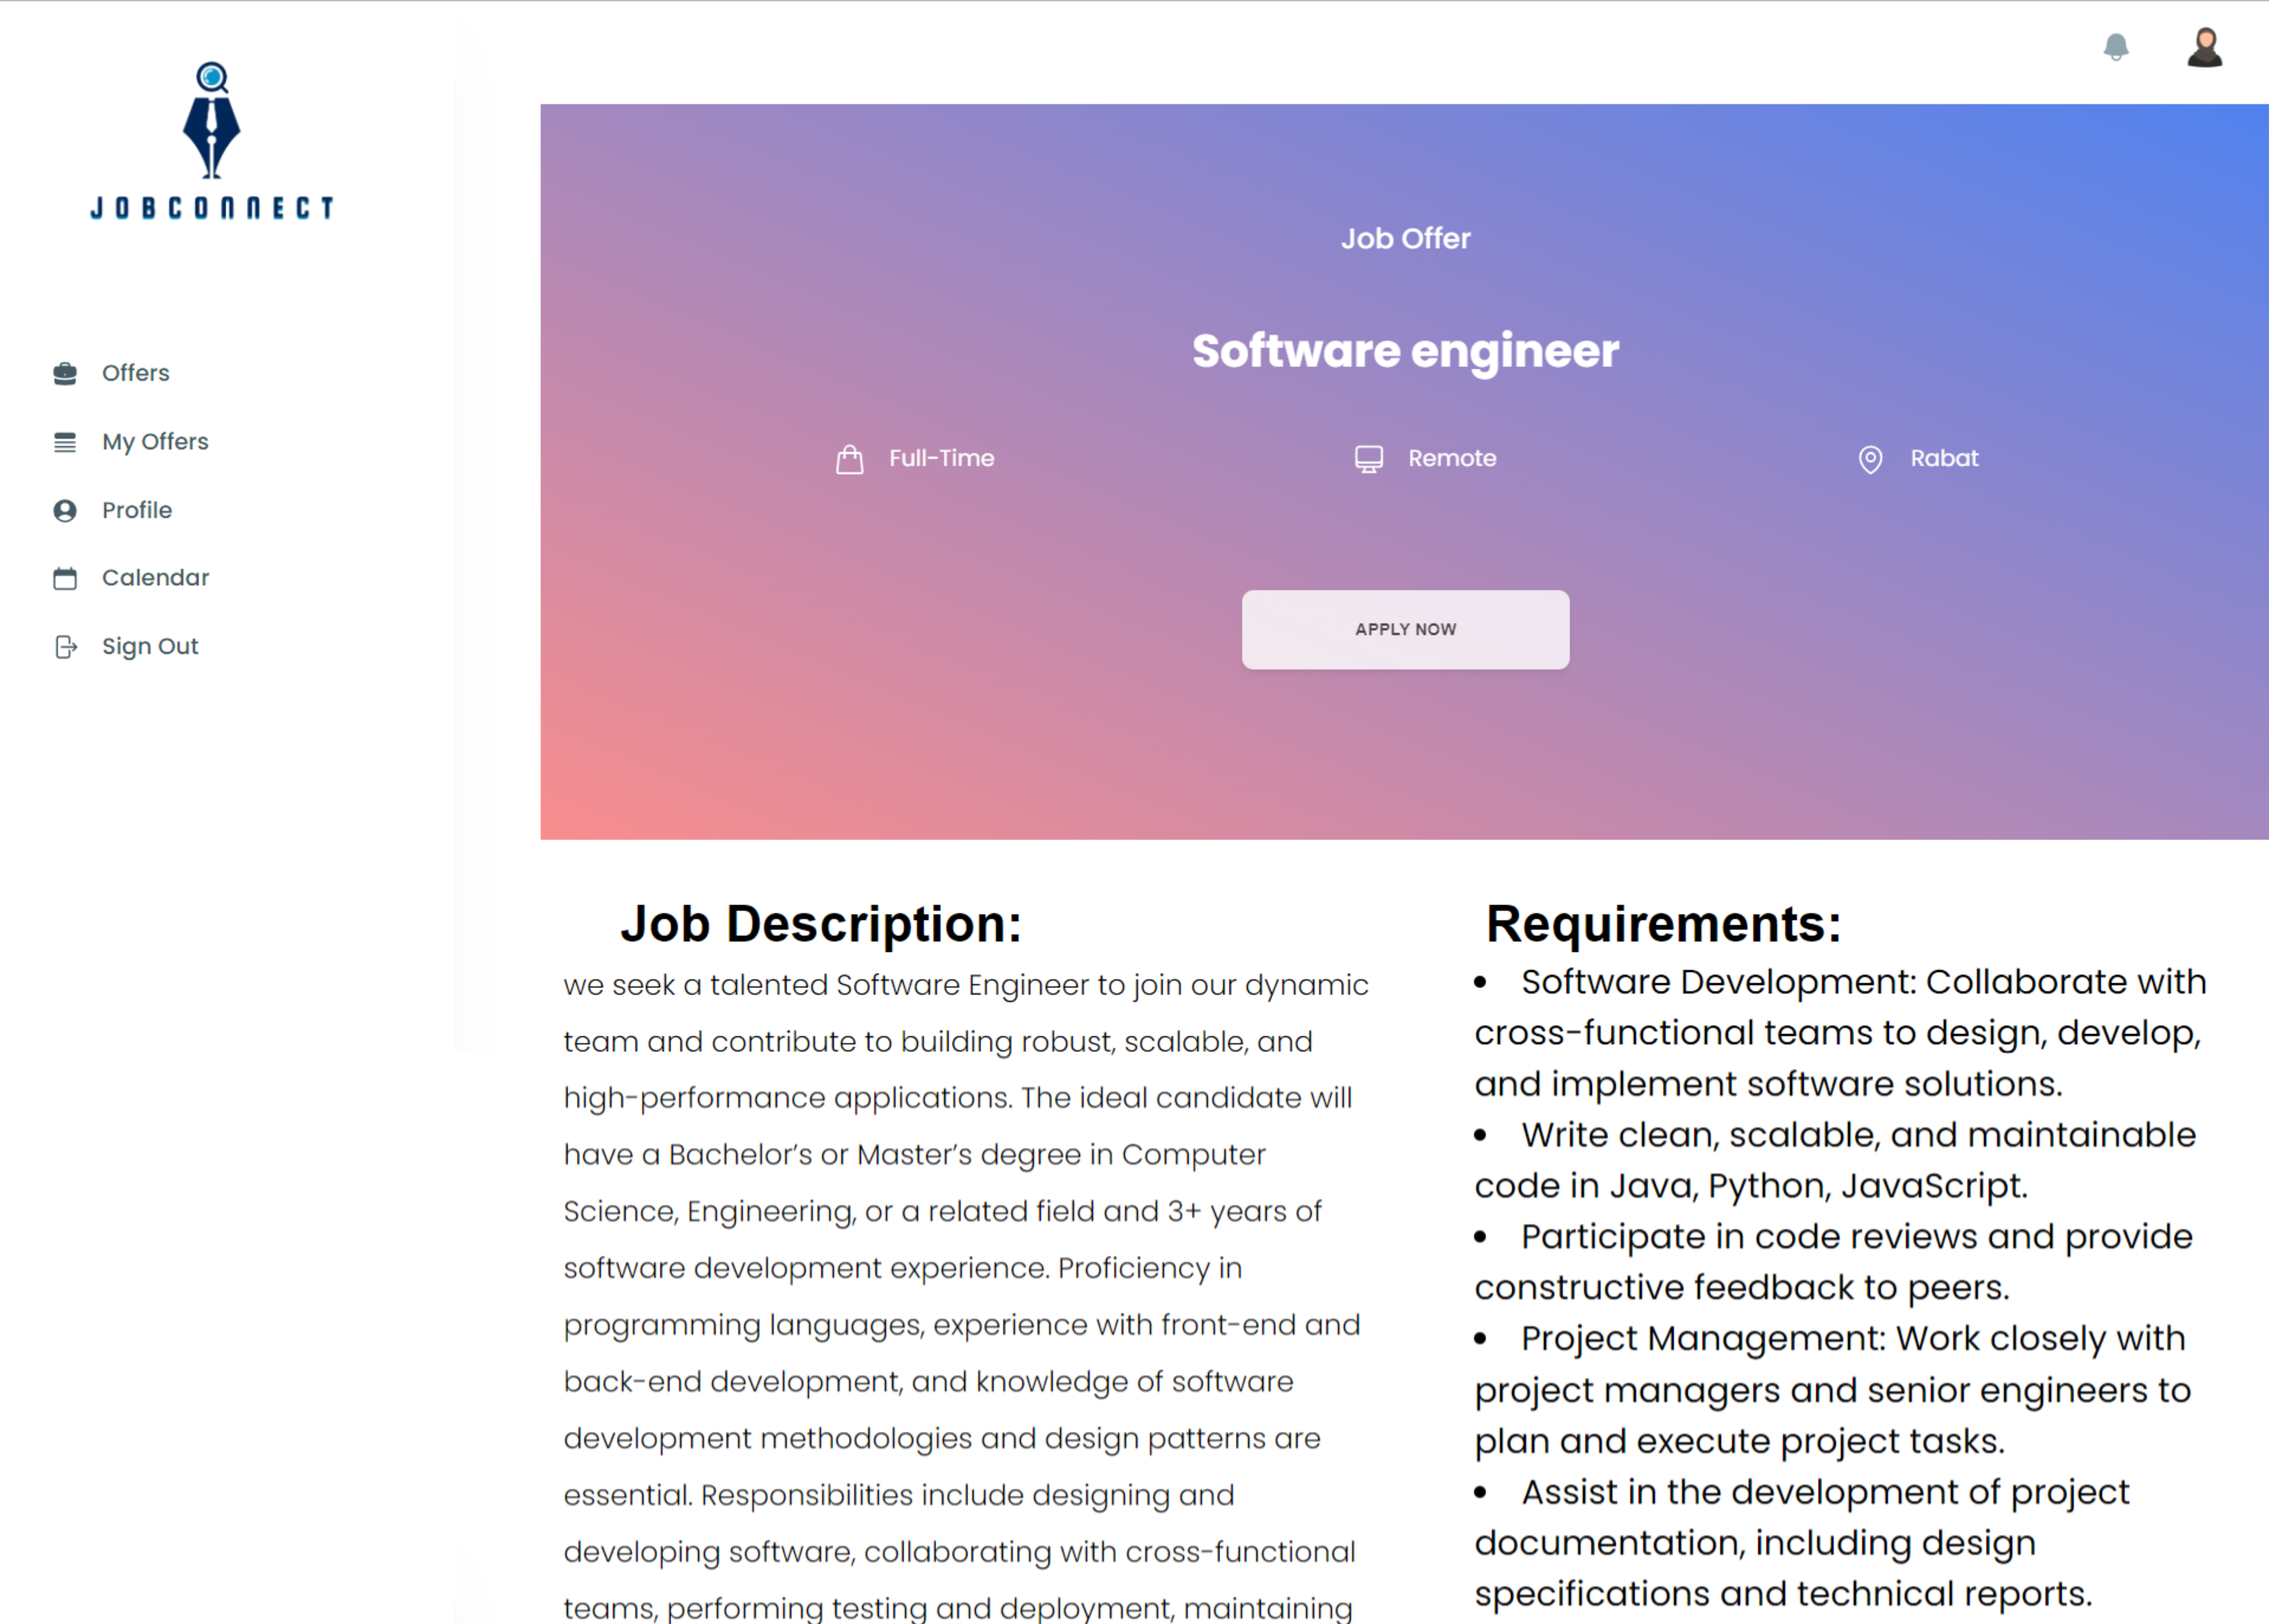
\includegraphics[scale=0.2]{screens/consultOffer.png} 
   \caption{Consulter le detail d'une offre}
   \label{fig:detailsOffre}
\end{figure}
\vspace{3cm}

Si le candidat souhaite postuler à l'offre, il peut cliquer sur le  bouton "APPLY NOW". Cela affichera une boîte de dialogue confirmant la candidature à l'offre, comme illustré dans la figure.
\newline
\begin{figure}[htbp]
   \centering
   \includegraphics[scale=0.2]{screens/confirmJob2.png} 
   \caption{Confirmation de candidature}
   \label{fig:listOffers}
\end{figure}
Une fois la candidature soumise, un nouvel enregistrement est créé dans la table "Candidature", en stockant les attributs "offer_ID"  et  "candidat_ID"  à partir de la session.
Ces enregistrements sont utilisés pour être visualisés par le candidat dans un tableau de bord, qui sera discuté dans  la prochaine section "Mes offres".

\subsubsection{Mes offres}
Chaque candidat peut visualiser ses candidatures en cliquant sur le bouton "My offers" situé dans le  menu de  gauche. En accédant à la page "Mes offres", les  offres auxquelles le  candidat a postulé sont affichées dans un tableau. Ce  tableau inclut le titre du poste, la date de  soumission à l'offre, le  lieu, le  statut de  l’offre ainsi qu'un bouton "Démarrer le test". Ce  bouton devient fonctionnel après le calcul du score du CV, effectué en backend. 
\begin{figure}[htbp]
   \centering
   \includegraphics[scale=0.3]{screens/myOffers.png} 
   \caption{Historique de candidatures}
   \label{fig:listOffers}
\end{figure}

\subsubsection{Passer le test}


\subsubsection{Consulter le calendrier}


\subsection{Espace Recruteur}
\subsubsection{Consulter le dashboard}

\subsubsection{Publier une offre}

\subsubsection{Programmer un entretien}


\subsection{Espace Administrateur}

\subsubsection{Consulter le dashboard}

\subsubsection{Ajouter un recruteur}

\section{Test et Validation}
\subsection{Tests unitaires}
Jest

\subsection{Tests de bout en bout}
\subsubsection{Définition et importance}

Dans le contexte de notre projet, le test end-to-end fait référence à une approche de test qui vise à évaluer le système dans son ensemble, en simulant
\newline 
les conditions réelles d’utilisation. Il s’agit d’un type de test qui vérifie le bon fonctionnement du système depuis le début jusqu’à la fin, en testant toutes les étapes intermédiaires et les  interactions entre les  composants. L’importance du test end-to-end dans notre projet réside dans sa capacité  à valider  la fonctionnalité globale du système et à identifier les problèmes d’intégration potentiels. En effectuant des tests end-to-end, vous pouvez vérifier si toutes les parties du système fonctionnent harmonieusement ensemble et satisfont les exigences spécifiées.
\newline
Ces tests permettent également d’évaluer  les  performances  du  système dans des scénarios réalistes, en tenant compte des conditions et des charges de travail typiques. Ils offrent une vision globale de la  qualité  du  système,  en mettant l’accent sur les fonctionnalités essentielles et les  cas  d’utilisation critiques pour les utilisateurs finaux. En résumé, le test end-to-end est essentiel dans votre projet pour s’assurer que toutes les parties du système fonctionnent correctement ensemble, répondent aux exigences et offrent une expérience utilisateur optimale. Il permet d’identifier et de résoudre les problèmes d’intégration pré- cocement, ce qui améliore la  qualité  du  produit  final.  La figure 77 montre le fonctionnement du test E2E par cypress.
\begin{figure}[htbp]
   \centering
   \includegraphics[scale=0.2]{screens/listOffers.png} 
   \caption{Liste des offres}
   \label{fig:listOffers}
\end{figure}



\subsubsection{Exemple sur la page d’authentification}

